\chapter{Verwandte Arbeiten} \label{sec:VerwandteArbeiten}
Im Folgenden werden Forschungsarbeiten vorgestellt, die sich mit Fragestellung beschäftigen, die den beiden zuvor vorgestellten Problemstellungen (siehe Abschnitt \ref{sec:Problemstellung}) ähnlich sind. Zunächst wird ein Überblick über Arbeiten gegeben, die sich mit dem Vergleich oder Vorstellung mehrerer Visualisierungstechniken beschäftigen. Anschließend werden Arbeiten vorgestellt, die sich speziell mit dem Treemap-Problem beschäftigen, also dem Problem von verschwindenden Knoten.

\section{Vergleich von Visualisierungstechniken} \label{sec:VergleichVisualisierungstechniken}

Die Arbeit von Pacione et al. (\textit{A comparative evaluation of dynamic visualisation tools} \cite{pacione2003comparative}) vergleicht fünf dynamische Visualisierungstools bezüglich ihrer Eignung für das Softwareverständnis und das Reverse Engineering. Die Autoren verfolgen das Ziel, Gründe dafür zu identifizieren, weshalb der Einsatz dieser Werkzeuge außerhalb der Forschung bislang nur begrenzt erfolgt, obwohl sie großes Potenzial für die Analyse komplexer Softwaresysteme bieten. Die Studie macht deutlich, dass keines der untersuchten Tools alle Anforderungen an Softwareverständnis vollständig abdeckt. Insbesondere wird auf Defizite in der Abbildung von Design-Patterns und Hotspot-Analysen hingewiesen, was unter Anderem im Kontext der Evaluation in dieser Arbeit untersucht werden soll.

Einen Überblick im Bereich der dreidimensionalen Softwarevisualisierung gibt die Arbeit von Teyseyre et al. (\textit{An overview of 3D software visualization} \cite{overview3D}). Die Autoren präsentieren verschiedene Visualisierungsansätze und Werkzeuge. Dabei werden folgende Kategorien differenziert:
\begin{itemize}
\item \textbf{Graphbasierte Ansätze:} 3D-Knoten-Kanten-Diagramme mit Fokus auf die Darstellung von Klassenbeziehungen
\item \textbf{Baumstrukturen:} Dreidimensionale Variationen wie \textit{Cone Trees}, \textit{Information Cubes} (im Grund 3D Treemaps) oder \textit{hierarchical nets} (siehe Abbildung \ref{fig:hierarchicalNet3D}) zur hierarchischen Darstellung von Softwareelementen
\item \textbf{Abstrakte Geometrische Darstellungen:} Nutzung von verschiedenen Formen zur Darstellung von verschiedenen Metriken und Strukturen. (Beispiel in Abbildung \ref{fig:geometrischeFiguren})
\end{itemize}
Sie zeigen auch auf, dass einige Ansätze Metaphern wie Städte oder Landschaften aus der echten Welt nutzen.
Interessant ist, dass von den 22 analysierten Tools nur vier für das Management oder Stakeholder ohne spezielle Entwicklungskompetenzen geeignet sind. Von diesen vier visualisiert zudem lediglich eines dieser Werkzeuge tatsächlich den Quellcode. Die anderen drei Tools konzentrieren sich auf die Visualisierung von Anforderungen. Zudem wird ein Mangel an empirischen Nutzungsstudien im 3D-Bereich konstatiert, was den Status und die Praxistauglichkeit der Ansätze weiter einschränkt. \cite{overview3D} In dieser Arbeit wird daher untersucht, ob die in dieser Arbeit vorgestellten Ansätze auch für Nutzer ohne tiefere technische Kenntnisse geeignet sind.

\begin{figure}
    \centering
    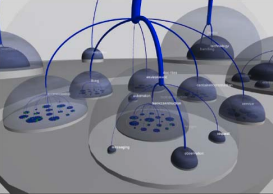
\includegraphics[width=0.8\textwidth]{images/verwandte/hierarchicalNet3D.png}
    \caption{Beispiel für ein hierarchisches Netz in 3D. Die hierarchische Struktur wird durch Kreise, Halbkugeln und deren Verbindungen dargestellt. \cite[6]{overview3D}}
    \label{fig:hierarchicalNet3D}
\end{figure}

\begin{figure}
    \centering
    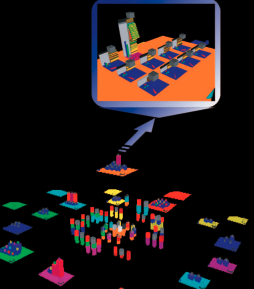
\includegraphics[width=0.8\textwidth]{images/verwandte/geometrischeFiguren.png}
    \caption{Beispiel für eine abstrakte geometrische Darstellung von Software. \cite[7]{overview3D}}
    \label{fig:geometrischeFiguren}
\end{figure}

Auch die Arbeit von Caserta und Zendra (\textit{Visualization of the static aspects of software: A survey} \cite{staticSurvey}) gibt einen Überblick über etablierte und aktuelle Visualisierungstechniken und ordnet diese unterschiedlichen Analyseebenen zu:
\begin{itemize}
\item \textbf{Quellcode-Ebene:} Zeilenorientierte Visualisierungen von einzelnen Dateien oder Klassen
\item \textbf{Klassen-/Mittel-Ebene:} Darstellungen der Strukturen oder Relationen von Dateien oder Klassen
\item \textbf{Architekturebene:} Globale Übersichten über Organisation und Qualitätsattribute, etwa durch Darstellung von Vererbungen und Aufrufstrukturen
\end{itemize}
Für die Architekturebene, die im Fokus dieser Arbeit steht, werden insbesondere folgende Visualisierungstypen diskutiert: Tree/Node-Link-Diagramme (wie Bereits in der Grundlagen gezeigt: bei großen Systemen schnell unübersichtlich), Treemaps und deren Varianten (Circular, Sunburst, Voronoi), die hierarchische Strukturen platzsparend repräsentieren und in 2D sowie 3D verfügbar sind. Sie stellen unter anderem folgende Probleme dieser Visualisierungen fest: Schlechte Nutzbarkeit, kognitive Überlastung, Desorientierung in dreidimensionalen Darstellungen sowie eine geringe Verbreitung praxistauglicher Tools, da viele existierende Lösungen im Prototypstatus sind.

Die Übersicht von Khan et al. (\textit{Visualization and evolution of software architectures} \cite{visualizationEvolution}) stellt ebenfalls verschiedene Visualisierungstechniken vor.
Sie unterscheiden zwischen hierarchischen und beziehungsorientierten Visualisationstechniken. Bei den hierarchischen Ansetzen werden platzfüllende Treemaps vorgestellt, die aufgrund ihrer Eigenschaften vor allem für große Hierarchien geeignet sind, wobei Sie hervorheben, dass Einschränkungen hinsichtlich der Visualisierung multipler Metriken und der Anschaulichkeit interner Strukturen bestehen, was in dieser Arbeit angegangen wird. Ergänzend nennen die Autoren auch Icicle Plots, Sunburst-Diagramme und hyperbolische Bäume (siehe Abbildung \ref{fig:dreiVis}).

\begin{figure}
    \centering
    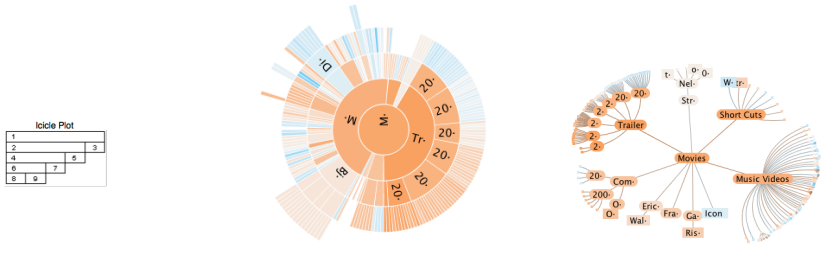
\includegraphics[width=0.8\textwidth]{images/verwandte/dreiVis.png}
    \caption{Beispiele für \textit{Icicle Plots} (links), \textit{Sunburst-Diagramme} (mitte) und \textit{hyperbolische Treelayouts} (rechts). \cite[4]{visualizationEvolution}}
    \label{fig:dreiVis}
\end{figure}

In \textit{Software visualization tools: survey and analysis} \cite{bassil2001software} von Bassil und Keller führen eine Umfrage durch, in der sie untersuchen, was Nutzern bei Softwarevisualisierungstools wichtig ist. Es zeigte sich, dass insbesondere hierarchische Repräsentationen, Benutzerfreundlichkeit und Skalierbarkeit bei großen Softwaresystemen von den Nutzern als entscheidend bewertet werden. Auch hier ist auffällig, dass speziell Experten befragt werden und sich auch die meisten untersuchten Werkzeuge primär an Experten und weniger an Endanwender wie Softwarekunden oder Management richten.

Eine detaillierte Übersicht verschiedener Treemap-Layout-Algorithmen geben Scheibel et al. in ihrer Arbeit \textit{Survey of treemap layout algorithms} \cite{scheibel2020survey}. Die Autoren unterscheiden Treemap-Algorithmen anhand der Art der Aufteilung (packing vs. splitting). Splitting ist die klassische Treemap-Variante, bei der die Fläche geteilt wird. Packing-Ansätze hingegen platzieren die Rechtecke so, dass sie möglichst wenig Platz verschwenden. Beide Ansätze erzeugen leicht Verschiedene Layouts (siehe Abbildung \ref{fig:packingVsSplitting}).  

\begin{figure}
    \centering
    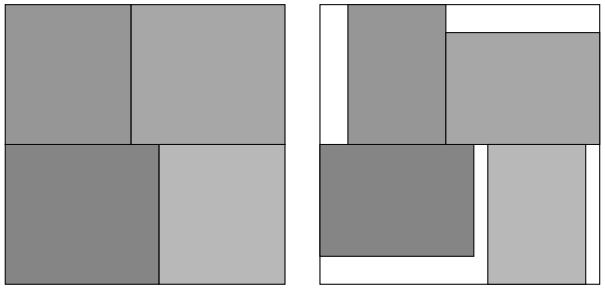
\includegraphics[width=0.8\textwidth]{images/verwandte/packingVsSplitting.png}
    \caption{Beispiel für Layouts die durch Splitting (links) und Packing (rechts) Algorithmen erzeugt wurden. Es ist zu erkennen, dass bei Packing-Algorithmen mehr Platz zwischen den Knoten entsteht. \cite[3]{scheibel2020survey}}
    \label{fig:packingVsSplitting}
\end{figure}

Zudem unterscheiden sie verschiedene layouts anhand der Layout-Form (z.,B. rechteckig, kreisförmig, konvex, nicht-konvex) sowie der Referenzraum-Dimension (2D vs. 3D). Für die in dieser Arbeit betrachteten Anwendungsfälle stehen rechteckige 2D-Splitting-Layouts im Vordergrund (siehe Abschnitt\ref{sec:Problemstellung} und \ref{sec:Treemap}) Wir stellen fest, dass von 81 analysierten Ansätzen sind 54 rechteckige und 58 splitting-basiert sind, was zeigt, dass dies das präferierte Treemap verfahren ist. 
Neben klassischen Verfahren (Slice-and-Dice, Squarified, Strip) werden auch Polygon-, Voronoi- und Circular-Treemaps sowie spezialisierte Layouts beschrieben, etwa für Aspektverhältnis-Optimierung oder Ordnungserhaltung. Die große Vielfalt verdeutlicht die Notwendigkeit einer gezielten anwendungsspezifischen Auswahl des Algorithmus.

\smallskip

Die analysierten Arbeiten verdeutlichen eine große Vielfalt an Visualisierungsansätzen für Softwaresysteme. Diese Vielfalt unterstreicht die Notwendigkeit eines vergleichenden Ansatzes, um die Stärken und Schwächen unterschiedlicher Techniken systematisch herauszuarbeiten. Zugleich wird in der Literatur fortwährend eine Diskrepanz zwischen den in der Forschung entwickelten Konzepten und deren tatsächlichem Einsatz in der Praxis festgestellt, da viele der vorgestellten Ansätze prototypischer Natur oder stark theoretisch ausgerichtet sind\cite{overview3D, staticSurvey}.

Darüber hinaus mangelt es an umfassenden empirischen Studien zur Evaluation dieser Ansätze. In einigen Arbeiten werden neue Visualisierungsmethoden beschrieben, ohne deren Wirksamkeit im Vergleich zu etablierten Methoden systematisch zu untersuchen \cite{overview3D, scheibel2020survey, visualizationEvolution}. Um die Praxisrelevanz zu erhöhen, berücksichtigt die vorliegende Arbeit auch existierende, in realen Kontexten eingesetzte Werkzeuge und legt einen besonderen Fokus auf die Bedürfnisse von Endnutzern und Stakeholdern, die in bisherigen Arbeiten häufig nur unzureichend adressiert wurden\cite{bassil2001software, pacione2003comparative}.


 


\section{Das Treemap-Problem}
Lü und Fogarty identifizieren in ihrer Arbeit \cite{lu2008cascaded} als zentrales Problem von Treemaps die erschwerte Wahrnehmbarkeit der zugrundeliegenden Hierarchiestruktur: \enquote{An important limitation of treemaps is the difficulty of discerning the structure of a hierarchy} \cite[1]{lu2008cascaded}. Dieses Problem wird auch in anderen Arbeiten als eine der größten Herausforderungen für algorithmische Treemap-Layouts genannt (siehe Abschnitt \ref{sec:TreemapProblem}). Verschiedene Ansätze in der Literatur beschäftigen sich mit diesem Problem.

Die Autoren des ursprünglichen Squarified-Treemap-Algorithmus \cite{bruls2000squarified} entwickeln in einer späteren Arbeit das Konzept der \textit{Cushion Treemaps} \cite{cushionTreemaps}. Dabei wird jedem Knoten ein Innenraumschatten zugewiesen, welcher durch gezielte Schattierungseffekte die hierarchische Struktur visuell hervorhebt (siehe Abbildung \ref{fig:cushion}). Auf diese Weise bleibt das klassische Layout erhalten, während die Wahrnehmung der Hierarchiebeziehungen unterstützt wird.

\begin{figure}
    \centering
    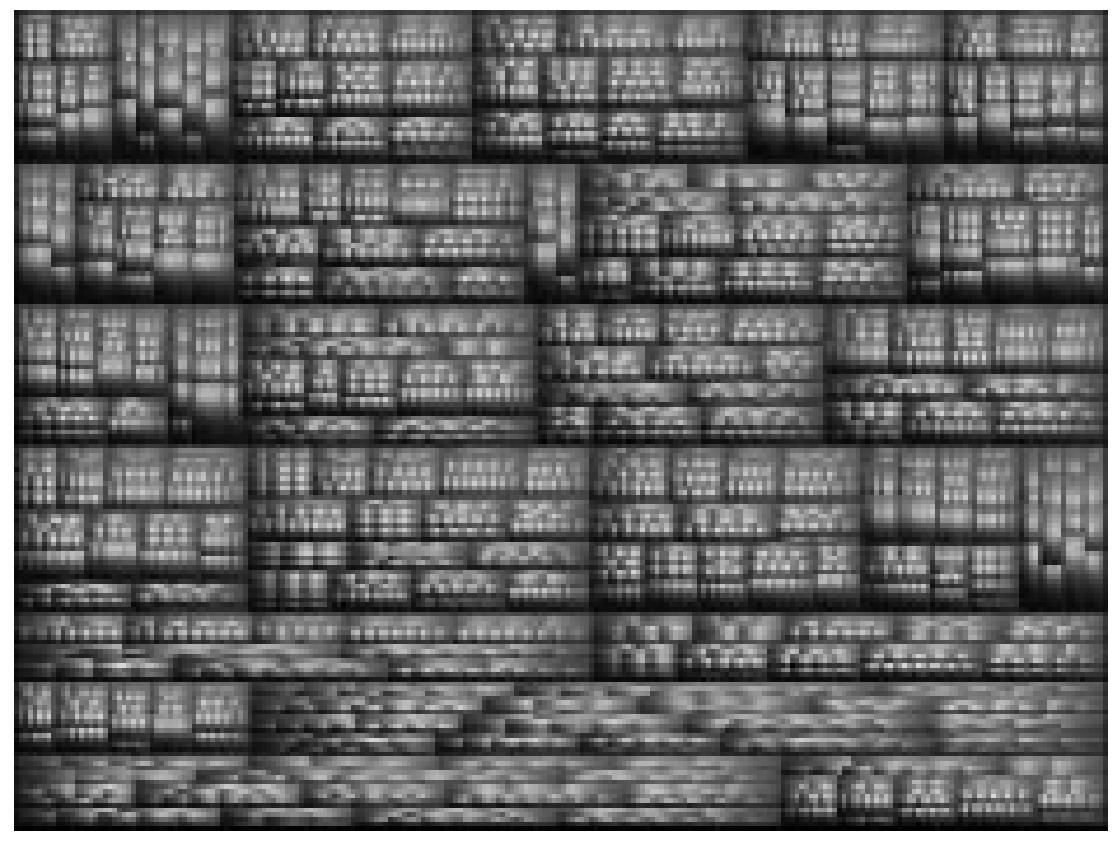
\includegraphics[width=0.8\textwidth]{images/cushionTreemap.png}
    \caption{Beispiel für eine Cushion Treemap \cite[4]{cushionTreemaps}.}
    \label{fig:cushion}
\end{figure}

Ein alternativer Ansatz wird von Demian und Fruchter präsentiert, indem sie die Verwendung unterschiedlich dicker Umrisslinien vorschlagen, um die Zugehörigkeit und Tiefe der Knoten in der Hierarchie hervorzuheben \cite{largeHierarchicalRepositories}. Ähnliches schlagen auch Kong et al. vor, die die Vor- und Nachteile verschiedener Umriss-Stärken für die Darstellung der Knotenstruktur vorstellen \cite{2010-perception-treemaps} (siehe Abbildung \ref{fig:thickOutline}).

\begin{figure}
    \centering
    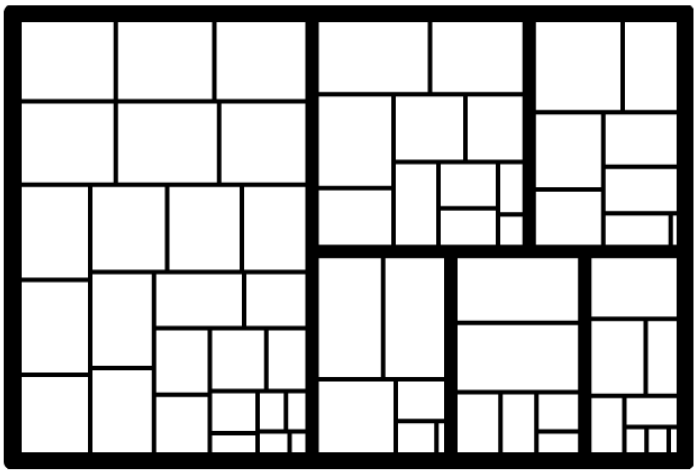
\includegraphics[width=0.8\textwidth]{images/lineThickness2.png}
    \caption{Beispiel für eine Treemap mit unterschiedlich dicken Outlines zur Verdeutlichung der Hierarchiestruktur der Knoten \cite[1]{2010-perception-treemaps}.}
    \label{fig:thickOutline}
\end{figure}

Obwohl diese Ansätze die Erkennbarkeit der Struktur in 2D signifikant verbessern, sind sie für Anwendungen im 2.5D- oder 3D-Kontext wenig geeignet, da Schatten und Outlines bei einer Extrusion ins Dreidimensionale nicht konsistent und flächenübergreifend darstellbar sind. Dies führt dazu, dass insbesondere bei 3D-Treemaps (Extrusion ohne zusätzliche Farbgebung) die hierarchische Struktur nur schwer erkannt werden kann. Daher besteht Bedarf an Layout-Algorithmen, die explizit räumliche Abstände zwischen den Hierarchieebenen erzeugen. Klassische Treemap-Layouts verzichten in der Regel auf solche Abstände, was die Lesbarkeit der Hierarchie in extrudierten Darstellungsformen weiter erschwert \cite{wood2008spatially, shneiderman2001ordered, hu2014squarified}.

Eine explizite Behandlung dieses Problems findet sich in der Arbeit \textit{Cascaded treemaps: examining the visibility and stability of structure in treemaps} \cite{lu2008cascaded} von Lü und Fogarty, die im Folgenden detailliert dargestellt wird. Die Arbeit von Lü und Fogarty bildet außerdem eine idee-gebende Grundlage für die in dieser Arbeit vorgenommenen Anpassungen am Squarified-Treemap-Algorithmus.

Im Gegensatz zu verschachtelten (\textit{Nested}) Ansätzen, bei denen Kindknoten streng innerhalb der Elternelemente platziert werden, schlagen Lü und Fogarty eine leichte Versetzung der Kindknoten vor. Diese werden im sogenannten \textit{Cascaded Treemap}-Ansatz nicht direkt innerhalb, sondern leicht versetzt \textit{über} ihren Elternknoten dargestellt (siehe Abbildung \ref{fig:cascaded}). Dadurch wird ein subtiler 3D-Effekt erzeugt und der Platzverlust im Vergleich zu klassischen Verschachtelungen reduziert.

\begin{figure}
    \centering
    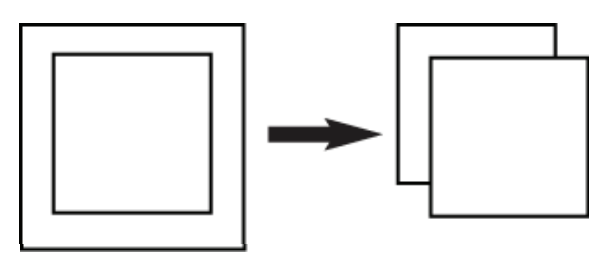
\includegraphics[width=0.8\textwidth]{images/cascaded.png}
    \caption{Links: Nested-Treemap-Ansatz mit vollständig platzierter Verschachtelung. Rechts: Der Cascaded-Treemap-Ansatz nach \cite[3]{lu2008cascaded} mit versetzten Kindknoten.}
    \label{fig:cascaded}
\end{figure}

Ein identifiziertes Problem bei diesem Verfahren (und auch bei klassischen Nested Layouts) besteht darin, dass Knoten vollständig verschwinden können, wenn nicht ausreichend Platz für Abstände und Beschriftungen zur Verfügung steht. Um dieses Problem abzumildern, schlagen Lü und Fogarty einen zweistufigen Prozess vor: Im ersten Schritt erfolgt eine Flächenaufteilung mittels des Squarified-Treemap-Algorithmus \cite{bruls2000squarified}. Im anschließenden zweiten Schritt werden für die einzelnen Knoten Abstände und Beschriftungsflächen neu berechnet, wobei die Größe, nicht jedoch die Position der Knoten angepasst wird. Dabei kann es, trotz dieses Verfahrens, weiterhin zum Verschwinden von Knoten kommen, wenn nicht genügend Raum für Beschriftung und Abstand vorhanden ist. Einen Pseudocode für die genaue Implementierung liefern die Autoren nicht, sodass eine Nachvollziehbarkeit und ein quantitativer Vergleich zu alternativen Algorithmen erschwert wird.

Das Verfahren wird wie folgt beschrieben:
\begin{quote}
    The function then computes how much vertical space is needed for offsets [...]. The remaining space is for the content of the treemap, and so the layout function gives each side of the split the space computed as necessary for [...] offsets as well as a portion of the remaining content space based on the relative weights of nodes on each side of the split. The layout procedure is then ready to recurse on both sides of the split, as it knows how much space will be used by [...] offsets and has ensured that the remaining space is appropriately divided by node weight. \cite[6]{lu2008cascaded}
\end{quote}

Für jeden Knoten wird die verfügbare Fläche jeweils neu berechnet. Dabei wird an jeder Teilungskante, der Kante, an der ein Knoten entweder horizontal oder vertikal aufgeteilt wird, die für Abstände benötigte Fläche bestimmt. Es wird also immer eine Reihen betrachtet. Zunächst erfolgt die Berechnung des PLatzes, der für die Abstände entlang dieser Teilungskante notwendig ist. Im Anschluss wird der verbleibende Raum für die eigentlichen Knoten berechnet, indem die Fläche für die Abstände von der Gesamtfläche subtrahiert wird. Auf diese Weise wird sichergestellt, dass für jeden Knoten ausreichend Platz für die erforderlichen Abstände eingeplant wird und die Knoten entsprechend ihrer Gewichtung skaliert sind. 

Allerdings bleibt ein zentrales Problem bestehen. Es kann dazu kommen, dass einzelne Knoten vollständig verschwinden, wenn der für die Abstände erforderliche PLatz größer ist als die für die Knoten verbleibende Fläche.
Das grundlegende Problem, das zuvor beschrieben wurde (siehe Abschnitt \ref{sec:TreemapProblem}), ist zwar dadurch weniger groß, aber nicht vollständig gelöst.

Obwohl kein Quellcode für das beschriebene Verfahren vorliegt, lässt sich basierend auf der publizierten Beschreibung ein weiterer Nachteil dieses Ansatzes erkennen: Bei jeder betrachteten Reihen-Kante wird nur der Raum für die Abstände entlang der Richtung berücksichtigt, die senkrecht zu dieser Kante steht. Abbildung \ref{fig:cascadedBadExample} veranschaulicht, dass der Algorithmus für den Bereich oberhalb und unterhalb der Trennlinie jeweils die gleiche Menge an Abstandfläche vorsieht, da ausschließlich die senkrechte Richtung zur Kante Berücksichtigung findet. Dies führt dazu, dass die in der Abbildung roten Rechtecke zusammen einen wesentlich größeren Bedarf an Abstand aufweisen würden als das gelbe Rechteck alleine. Der Algorithmus differenziert jedoch nicht zwischen diesen verschiedenen Konstellationen, was eine ineffiziente Allokation von Abstandflächen zur Folge haben kann.

\begin{figure}
    \centering
    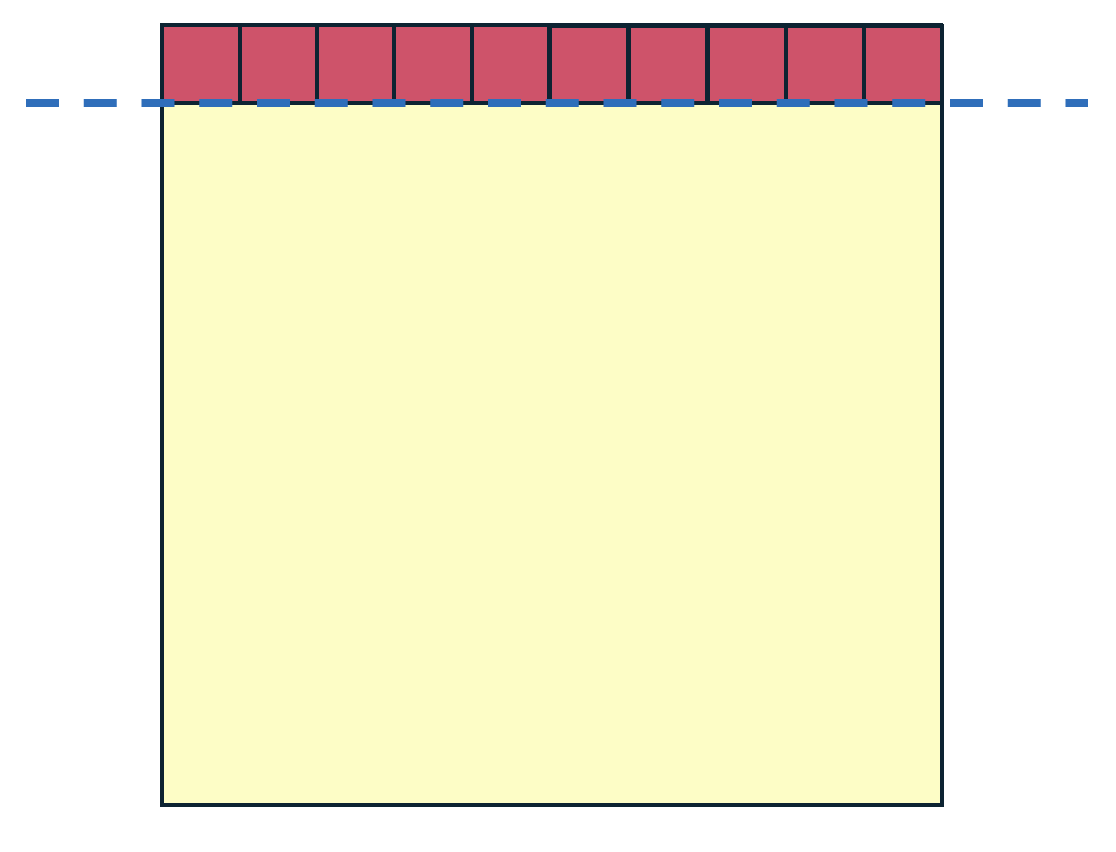
\includegraphics[width=0.8\textwidth]{images/cascadedBadExample.png}
    \caption{Illustration einer, für den den Cascaded-Treemap-Algorithmus, ungünstigen Flächenaufteilung. Die Teilungskante ist in blau gekennzeichnet. Senkrecht zu dieser Kante werden die Benötigten Flächen neu berechnet. Für die roten Rechtecke wird zu viel, für das gelbe Rechteck jedoch vergleichsweise wenig Abstand berücksichtigt.}
    \label{fig:cascadedBadExample}
\end{figure}


Lü und Fogarty berichten, dass mit ihrem Verfahren keine Verbesserung im Verhältnis von Knoten-Gewicht zu Knotengröße festgestellt werden konnte. Verbesserungen traten lediglich bei sehr kleinen Knoten auf, da konstante Abstände bei kleinen Flächen proportional stärker ins Gewicht fallen als bei größeren. Sie führen dies explizit auf ihren spezifischen Ansatz zurück und regen weiterführende Forschung zu diesem Problem an, was wir unter anderem in dieser Arbeit bezwecken. Darüber hinaus vermuten sie, dass die Abweichung zwischen Größen- und Gewichtsverhältnis in tiefen Hierarchien weiter zunimmt.
